\documentclass[journal,12pt,twocolumn]{IEEEtran}

\usepackage{setspace}
\usepackage{gensymb}
\singlespacing
\usepackage[cmex10]{amsmath}

\usepackage{amsthm}

\usepackage{mathrsfs}
\usepackage{txfonts}
\usepackage{stfloats}
\usepackage{bm}
\usepackage{cite}
\usepackage{cases}
\usepackage{subfig}

\usepackage{longtable}
\usepackage{multirow}
\usepackage{enumitem}
\usepackage{mathtools}
\usepackage{steinmetz}
\usepackage{tikz}
\usepackage{circuitikz}
\usepackage{verbatim}
\usepackage{tfrupee}
\usepackage[breaklinks=true]{hyperref}
\usepackage{graphicx}
\usepackage{tkz-euclide}

\usetikzlibrary{calc,math}
\usepackage{listings}
    \usepackage{color}                                            %%
    \usepackage{array}                                            %%
    \usepackage{longtable}                                        %%
    \usepackage{calc}                                             %%
    \usepackage{multirow}                                         %%
    \usepackage{hhline}                                           %%
    \usepackage{ifthen}                                           %%
    \usepackage{lscape}     
\usepackage{multicol}
\usepackage{chngcntr}

\DeclareMathOperator*{\Res}{Res}

\renewcommand\thesection{\arabic{section}}
\renewcommand\thesubsection{\thesection.\arabic{subsection}}
\renewcommand\thesubsubsection{\thesubsection.\arabic{subsubsection}}

\renewcommand\thesectiondis{\arabic{section}}
\renewcommand\thesubsectiondis{\thesectiondis.\arabic{subsection}}
\renewcommand\thesubsubsectiondis{\thesubsectiondis.\arabic{sub subsection}}


\hyphenation{optical networks semiconduc-tor}
\def\inputGnumericTable{}                                 %%

\lstset{
%language=C,
frame=single, 
breaklines=true,
columns=fullflexible
}
\date{March 2021}

\begin{document}

\newcommand{\BEQA}{\begin{eqnarray}}
\newcommand{\EEQA}{\end{eqnarray}}
\newcommand{\define}{\stackrel{\triangle}{=}}
\bibliographystyle{IEEEtran}
\raggedbottom
\setlength{\parindent}{0pt}
\providecommand{\mbf}{\mathbf}
\providecommand{\pr}[1]{\ensuremath{\Pr\left(#1\right)}}
\providecommand{\qfunc}[1]{\ensuremath{Q\left(#1\right)}}
\providecommand{\fn}[1]{\ensuremath{f\left({#1}\right)}}
\providecommand{\e}[1]{\ensuremath{E\left(#1\right)}}
\providecommand{\sbrak}[1]{\ensuremath{{}\left[#1\right]}}
\providecommand{\lsbrak}[1]{\ensuremath{{}\left[#1\right.}}
\providecommand{\rsbrak}[1]{\ensuremath{{}\left.#1\right]}}
\providecommand{\brak}[1]{\ensuremath{\left(#1\right)}}
\providecommand{\lbrak}[1]{\ensuremath{\left(#1\right.}}
\providecommand{\rbrak}[1]{\ensuremath{\left.#1\right)}}
\providecommand{\cbrak}[1]{\ensuremath{\left\{#1\right\}}}
\providecommand{\lcbrak}[1]{\ensuremath{\left\{#1\right.}}
\providecommand{\rcbrak}[1]{\ensuremath{\left.#1\right\}}}
\theoremstyle{remark}
\newtheorem{rem}{Remark}
\newcommand{\sgn}{\mathop{\mathrm{sgn}}}
\newcommand{\comb}[2]{{}^{#1}\mathrm{C}_{#2}}
\providecommand{\abs}[1]{\vert#1\vert}
\providecommand{\res}[1]{\Res\displaylimits_{#1}} 
\providecommand{\norm}[1]{\lVert#1\rVert}
%\providecommand{\norm}[1]{\lVert#1\rVert}
\providecommand{\mtx}[1]{\mathbf{#1}}
\providecommand{\mean}[1]{E\sbrak{ #1 }}
\providecommand{\fourier}{\overset{\mathcal{F}}{ \rightleftharpoons}}
%\providecommand{\hilbert}{\overset{\mathcal{H}}{ \rightleftharpoons}}
\providecommand{\system}{\overset{\mathcal{H}}{ \longleftrightarrow}}
	%\newcommand{\solution}[2]{\textbf{Solution:}{#1}}
\newcommand{\solution}{\noindent \textbf{Solution: }}
\newcommand{\cosec}{\,\text{cosec}\,}
\providecommand{\dec}[2]{\ensuremath{\overset{#1}{\underset{#2}{\gtrless}}}}
\newcommand{\myvec}[1]{\ensuremath{\begin{pmatrix}#1\end{pmatrix}}}
\newcommand{\mydet}[1]{\ensuremath{\begin{vmatrix}#1\end{vmatrix}}}
\numberwithin{equation}{subsection}
\makeatletter
\@addtoreset{figure}{problem}
\makeatother
\let\StandardTheFigure\thefigure
\let\vec\mathbf
\vspace{3cm}
\title{EE3900 Assignment - 4}
\author{Adhvik Mani Sai Murarisetty - AI20BTECH11015}
\maketitle
\newpage
\bigskip
\renewcommand{\thetable}{\theenumi}

Download latex-tikz codes from 
%
\begin{lstlisting}
https://github.com/adhvik24/EE3900/blob/main/Assignment_4/Assignment4.tex
\end{lstlisting}
%
Download python codes from 
%
\begin{lstlisting}
https://github.com/adhvik24/EE3900/blob/main/Assignment_4/Assignment4.py
\end{lstlisting}
\section{Linear forms qn 2.17}
A line perpendicular to the line segment joining
the points$\myvec{1\\0}$ and $\myvec{2\\3}$ divides it in the ratio
1 : n. Find the equation of the line.
\section{SOLUTION}
Let $\vec{M}$ be the midpoint of two points $\vec{A}=\myvec{1\\0}$ and $\vec{B}=\myvec{2\\3}.$
\begin{align}
    \vec{M}=\frac{n\vec{A}+\vec{B}}{n+1}=\frac{n\myvec{1\\0}+\myvec{2\\3}}{n+1}\\
    \implies\vec{M}=\frac{1}{n+1}\myvec{n+2\\3}\nonumber
\end{align}
The direction vector of line AB is
\begin{align}
    \myvec{1\\0}-\myvec{2\\3}=\myvec{-1\\-3}
\end{align}
The direction vector of line AB is normal vector of perpendicular line. Then
\begin{align}
    \vec{n}=\myvec{-1\\-3}
\end{align}
The equation of line in terms of normal vector is then obtained as
\begin{align}
    \vec{n}^T(\vec{x}-\vec{M})&=0\\
    \implies\myvec{-1&-3}&\brak{\vec{x}-\frac{1}{n+1}\myvec{n+2\\3}} = 0\\
    \therefore \myvec{-1&-3}\vec{x}&= \frac{-n-11}{n+1}
\end{align}
We got equation of the line perpendicular to line segment joining points $\vec{A}$ and $\vec{B}$ and dividing them in the ratio $1:n$. 

For plotting let us take $n = 2$, Then the perpendicular line equation will be as,
\begin{align}
    \myvec{-1&-3}\vec{x}&= \frac{-13}{3}
\end{align}
And the graph looks like,
\begin{figure}[htp]
    \centering
    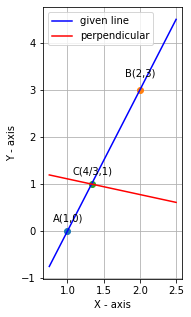
\includegraphics[width=\columnwidth]{a_4.png}
    \caption{graphical interpretation}
    \label{1}
\end{figure}
\end{document}
